

%\newcommand*{\ACM}{}%

\ifdefined\ACM

%\documentclass[sigplan,screen]{acmart}
  \documentclass[manuscript,screen,review]{acmart}

\else
  \documentclass{article}
  \usepackage{libertine}
  \usepackage[utf8]{inputenc}
\usepackage[a4paper, total={6in, 9in}]{geometry}
\usepackage{braket}
\usepackage{xcolor}
\usepackage{amsmath}
\usepackage{amsfonts}
\usepackage{amsthm}
\usepackage{amssymb}
%\usepackage[ocgcolorlinks]{hyperref}
\usepackage{hyperref}
%\usepackage{hyperref,xcolor}
%\usepackage[ocgcolorlinks]{ocgx2}
\usepackage{cleveref}
\usepackage{graphicx}
\usepackage{svg}
\usepackage{float}
\usepackage{tikz}
\usetikzlibrary{patterns, shapes.arrows}
\usepackage{adjustbox}
%\usepackage{tikz-network}
\usepackage{tkz-graph}
\usepackage{tkz-berge}
\usepackage[linesnumbered]{algorithm2e}
\usepackage{multicol}
\usepackage[backend=biber,style=alphabetic,sorting=ynt]{biblatex}
%\usepackage{xcolor}
%\usepackage{tkz-berge}
%\usepackage{tkz-graph}
\usepackage{pgfplots}
\usepackage{sagetex}
\usepackage{setspace}
\usepackage{etoc}
%\usepackage{wrapfig}
\usepackage{pgfgantt}
\DeclareUnicodeCharacter{2212}{−}
\usepgfplotslibrary{groupplots,dateplot}
\pgfplotsset{compat=newest}

\newtheorem{theorem}{Theorem}
\newtheorem{definition}{Definition}
\newtheorem{example}{Example}
\newtheorem{claim}{Claim}
\newtheorem{fact}{Fact}
\newtheorem{remark}{Remark}
\newtheorem*{theorem*}{Theorem}
\newtheorem{lemma}{Lemma}
\crefname{lemma}{Lemma}{Lemmas}
\hypersetup{colorlinks=true}
% , allcolors=blue,allbordercolors=blue,pdfborderstyle={0 0 1}}
%\hypersetup{pdfborder={2 2 2}}
% pdfpagemode=FullScreen,
% backref 

\newtheorem{problem}{Problem}
\crefname{problem}{Problem}{Problems}

\DeclareMathOperator{\Ima}{Im}


  \usepackage{cancel}
  \usepackage{subcaption}
  \addbibresource{./sample.bib} 

\fi

\begin{document}
\newcommand{\commentt}[1]{\textcolor{blue}{ \textbf{[COMMENT]} #1}}
\newcommand{\ctt}[1]{\commentt{#1}}
\newcommand{\prb}[1]{ \mathbf{Pr} \left[ #1 \right]}
\newcommand{\prbm}[2]{ \mathbf{Pr}_{ #2 }\left[ #1 \right]}
\newcommand{\prbc}[3]{ \mathbf{Pr}_{ #2 }\left[ #1 \right | #3]}
\newcommand{\prbcprb}[3]{ \prbc{#2}{#1}{#3} \cdot \prb{#3} } 
\newcommand{\expp}[1]{ \mathbf{E} \left[ {#1} \right]}
\newcommand{\onotation}[1]{\(\mathcal{O} \left( {#1}  \right) \)}
\newcommand{\ona}[1]{\onotation{#1}}
\newcommand{\PSI}{{\ket{\psi}}}
\newcommand{\xij} { X_{ij} } 
\DeclareMathOperator{\Ima}{Im}
%\newcommand{\LESn}{\ket{\psi_n}}
%\newcommand{\LESa}{\ket{\phi_n}}
%\newcommand{\LESs}{\frac{1}{\sqrt{n}}\sum_{i}{\ket{\left(0^{i}10^{n-i}\right)^{n}}}}
%\newcommand{\Hn}{\mathcal{H}_{n}}
%\newcommand{\Ep}{\frac{1}{\sqrt{2^n}}\sum^{2^n}_{x}{ \ket{xx}}}
%\newcommand{\HON}{\ket{\psi_{\text{honest}}}}
%\newcommand{\Lemma}{\paragraph{Lemma.}}
\newcommand{\Cpa}{[n, \rho n, \delta n]}
%\setlength{\columnsep}{0.6cm}
\newcommand{\Jvv}{ \bar{J_{v}} } 
\newcommand{\Cvv}{ \tilde{C_{v}} } 

\newcommand{\Gz}{ G_{z}^{\delta} } 
\newcommand{ \Tann } {  \mathcal{T}\left( G, C_0 \right) }
\newcommand{\ireducable}{ireducable \hyperref[ire]{[\ref{ire}]} }
\newcommand{\cutUU}{E(U_{-1} \bigcup U_{+1} ,U)} 
\newcommand{\wcutUU}{w\left( E(U_{-1} \bigcup U_{+1} ,U)  \right)}
\newcommand{\testgo}{  \mathcal{T}\left(J, q , C_{0}\right) } 

\newcommand{\duC}{\left( C_{A}^{\perp}\otimes C_{B}^{\perp} \right)^{\perp}}
\newcommand{\duduC}{\left( C_{A}\otimes C_{B}\right)^{\perp}}
  




\title{Magic States Distillation Using Quantum LDPC Codes. } 
\author{David Ponarovsky}
\maketitle




%\begin{abstract}
%  We studies the complexity of synthesis quantum states using PRS, our reasch continues the work by \cite{searchtodecision}, \cite{rosenthal2023efficient}, \cite{rosenthal2021interactive}, \cite{metger2023stateqip}, \cite{delavenne2023quantum}.
%\end{abstract}
%
%

\section{Good Codes With Large $\Lambda$.}
\newcommand*{\DETAILS}{}
\ifdefined\DETAILS


  \begin{claim}
    \label{claim:find}
    Let $v_{1},v_{2}..v_{k}$ vectors in $\mathbb{F}_{2}^{n}$, then there are $u_{1},u_{2}..u_{k^{\prime}}$ for $k^{\prime} > k/2$. Such $\text{ span } \{   u_{1},u_{2}..u_{k^{\prime}} \} \subset \text{ span } \{ v_{1},v_{2}..v_{k} \}$ and for any $i,j$ it holds that $u_{i}u_{j} = 0$. 
  \end{claim}
  \begin{proof}
    Consider the follow algorithm, 

    \begin{algorithm}[H]
      \caption{ Find commuted vectors $u_{1}, u_{2}, .. u_{k^{\prime}}$  }
      \label{alg:pick}
      Let $ J \leftarrow \emptyset$ \\
      \For{$i \in [k/2]$}{
        $J \leftarrow J \cup \{v_{2i-1}, v_{2i}\}$ \\
        \For{ $S \subset J$ }{
          Compute the vector $m_{S}$ define as $m_{S,j} = u_{j} \sum_{w\in S}w$
        }
        Pick $S$ such $m_{S} = 0$ and set $u_{i} \leftarrow  \sum_{w\in S}w$ \\ 
        Choose randomly $w \in S$ and set $J \leftarrow J/w$
      }
    \end{algorithm}
    \\
Now, we are going to prove that \Cref{alg:pick} always finds a subset $S$ that satisfies the equality on line (7). Assume not. On one hand, the number of possible values that $m_{S}$ can have is $2^{i} - 1$. On the other hand, since $J$ contains $i+1$ vectors on the $i$th iteration, it follows that the number of subsets is 
    \begin{equation*}
      \begin{split}
        2^{i+1}-1 \ge 2^{i}
      \end{split}
    \end{equation*}
Therefore, there must be at least two different subsets $S$ and $S^{\prime}$ such that $u_{S}=u_{S^{\prime}}$. However, this means that 
    \begin{equation*}
      \begin{split}
      m_{S\Delta S^{\prime}, j} = u_{j} \sum_{w\in S\Delta S^{\prime}}w = u_{j}\left(  \sum_{w\in S\Delta S^{\prime}}w + 2 \sum_{w \in S\cap S^{\prime}}w\right) = m_{S,j} +m_{S^{\prime},j} = 0 
      \end{split}
    \end{equation*}
Thus, $m_{S\Delta S^{\prime}} = 0$. Additionally, it is clear that the rank does not decrease, as for $u_{i}$, there exists one $v_{j}$ such that only $u_{i}$ is supported by $v_{j}$.
  \end{proof}

  \begin{claim}
    Let $v_{1},v_{2}..v_{k}$ vectors in $\mathbb{F}_{2}^{n}$, then there are $u_{1},u_{2}..u_{k^{\prime}}$ for $k^{\prime} > k/4$. Such $\text{ span } \{   u_{1},u_{2}..u_{k^{\prime}} \} \subset \text{ span } \{ v_{1},v_{2}..v_{k} \}$. And for any $i,j$ $\sum u_{i,k}u_{j,k} =_{4} 0$. 
  \end{claim}
\begin{proof}
Use the \Cref{alg:pick} twice. However, in the second iteration, define $m_{S,j}$ to be the product of module 4. Note that $m_{S,j}$ must be either $4n$ or $4n+2$. Thus, we can follow the proof of \Cref{claim:find}.
\end{proof}

  \begin{figure}[h]
\begin{subfigure}[t]{0.65\textwidth}
\begin{definition}
  Let $M \in \mathbb{F}_{2}^{k \times n }$ upper triangular matrix such that~$k~<~n$. We say that $M$ has the $1$-stairs property if $M_{ij}=1$ any $j<i$. 
\end{definition}
\begin{claim}
  \label{claim:stair}
  Any $M \in \mathbb{F}_{2}^{k \times n }$ upper triangular matrix can be turn into upper triangular matrix that has the $1$-stairs property by elementary operation.  
\end{claim}

\end{subfigure}
\begin{subfigure}[t]{0.05\textwidth}
  \
\end{subfigure}
  \begin{subfigure}[t]{0.25\textwidth}

    \begin{equation*}
      \begin{split}
        \begin{bmatrix}
         1 & 1 & 1 &1 &1 &\cdot & \cdot & \cdot & \cdot & \cdot \\     
         0 & 1 & 1 &1 &1 &\cdot & \cdot & \cdot & \cdot & \cdot \\     
         0 & 0 & 1 &1 &1 &\cdot & \cdot & \cdot & \cdot & \cdot \\     
         0 & 0 & 0 &1 &1 &\cdot & \cdot & \cdot & \cdot & \cdot \\
         0 & 0 & 0 &0 &1 &\cdot & \cdot & \cdot & \cdot & \cdot 
        \end{bmatrix}
      \end{split}
    \end{equation*}

 \end{subfigure}
\end{figure}
\begin{proof} 
Consider the following algorithm: Let $M$ be our initial matrix. We iterate over the rows from left to right. In the $i$th iteration, we check for any row $j<i$ if $M_{ji} = 1$. If not, we set $M$ to be the matrix obtained by adding the $i$th row to the $j$th row. Since $M$ is an upper triangular matrix, adding the $i$th row does not change any entry $M_{js}$ for $s<i$. Therefore, the obtained matrix is still an upper triangular matrix and the entries at $M_{js}$ for $j,s < i$ remain the same, namely $1$ if and only if $j\le s$. 

Continuing with the process eventually yields, after $k$ iterations, a matrix with the $1$-stair property.
\end{proof}


\fi

\begin{claim} 
  \label{claim:commute}
  Let $C$ be a $[n,k,d]$ binary linear code, and let $\Lambda$ be subcode $\Lambda \subset C$ at dimension $k' > \alpha k$ for some $\alpha\in(0,1)$. Then there exists a code $C' = [\leq 2n, \geq (1 - \alpha + \frac{\alpha^{3}}{24})k, d]$ and a subcode of it $\Lambda' $ in it at dimension $\ge \frac{\alpha^{3}}{24}k$, such:
  \begin{enumerate}
      \label{property:prop}
    \item For every $x \in \Lambda'$ and $y \in C^{\prime} \ \ x\cdot y = 0$
    \item For every $x \in \Lambda'$ and $y,z \in C^{\prime} \ \ x \cdot y \cdot z =0 $
  \end{enumerate}
\end{claim}
\begin{proof} 
  First, we can assume that the generator matrix of $C$ is an upper triangular matrix, such that the first $k^\prime$ rows span $\Lambda$. Notice that after applying the algorithm from \Cref{claim:stair} starting from the first row and stopping at the $k^{\prime}$th row, the first $k^{\prime}$ rows are kept in $\Lambda$. So let's assume that is the form of the generator matrix. 

  
  Now, let's consider the following process: going uphill, from right to left, starting at the $k^\prime$ row. Initially, set $j \leftarrow k^{\prime}$ and in each iteration, advance it to be the index of the next row, namely $j\leftarrow j - 1$. In each iteration, ask how many rows $G_{m}$, such that $m \le j$, satisfy $G_{m} G_{j} = 0$ and how many pairs of rows $G_{m},G_{m^{\prime}}$ such that $m,m^{\prime}\le j$ satisfy $G_{m}\cdot G_{m^{\prime}} \cdot G_{j} = 0$. Denote by $p$ the probability to fall on unsatisfied equation from the above.  
  \begin{itemize}
    \item If $p \ge \frac{1}{2}$ then we move on to the next iteration. 
    \item Otherwise, we encode the $j$th coordinate by $C_{0}$, which maps $1 \rightarrow w$ such that $w\cdot w = 0$. This flips the value of $G_{m} G_{j}$ for any pair and $G_{m} G_{m^{\prime}} G_{j}$ for any triple such that $m,m^{\prime} \le j$, so we get that the majority of the equations are satisfied. Also notice that the concatenation doesn't change the value of any multiplication at the form $G_{m}G_{j^{\prime}}$ for $j^{\prime}> j$. Therefore, for any $j< j^{\prime}\le k^{\prime}$ the number of the satisfied equations relative to $j^{\prime}$ is not changed, meaning it is still the majority.

      Set $G$ to be the new matrix after the concatenation by $C_{0}$.
  \end{itemize}

  In the end of the process $G$ is going to be the generator matrix of $C^{\prime}$. It's left to construct $\Lambda^{\prime}$, we are going to do so by taking from the $k^{\prime}$ rows a subset that satisfies the desired property in \Cref{property:prop}. 

Let $S$ be the set of rows among the first $k^{\prime}$ rows for which there is at least one unsatisfied equation. We will now prove that if $k^{\prime}$ is large enough, specifically linear in $k$, then $|S|$ is small enough to obtain $\Lambda^{\prime}$ by removing the rows in $S$.

Observe that the number of satisfied equations is at least:
  \begin{equation*}
    \begin{split}
      & \frac{1}{2}\left(k^{\prime}-1+(k^{\prime}-1)^{2}\right)  +\frac{1}{2}\left(k^{\prime}-1+(k^{\prime}-1)^{2}\right)  +\frac{1}{2}\left(k^{\prime}-2+(k^{\prime}-2)^{2}\right)  + .. +\frac{1}{2}\left(1+( 1 )^{2}\right) \\ 
      & = \frac{1}{2} \left(  { k^{\prime} + 1 \choose 2 }  + \frac{k^{\prime}(k^{\prime}+1)(2k^{\prime}+1)}{6} \right) 
    \end{split}
  \end{equation*}
  So 
  \begin{equation*}
    \begin{split}
      |S| \cdot k + |S|\cdot k^{2}  & \le  k^{\prime} \left( k + k^{2} \right) - \frac{1}{2} \left(  { k^{\prime} + 1 \choose 2 }  + \frac{k^{\prime}(k^{\prime}+1)(2k^{\prime}+1)}{6} \right) 
\\
\Rightarrow & |S| < k^{\prime} - \frac{1}{2}\left( \frac{1}{k^{2}+k} { k^{\prime} + 1 \choose 2 }  + \frac{1}{k^{2}+k} \frac{k^{\prime}(k^{\prime}+1)(2k^{\prime}+1)}{6} \right) \\
\Rightarrow & |S| < k^{\prime} - \frac{k^{\prime 3}}{24k^{2}} <k^{\prime} - \alpha^{2}\frac{k^{\prime} k^{2}}{24k^{2}} 
    \end{split}
  \end{equation*}

  Therefore, if $k^{\prime} \ge  \alpha k$ we have that $|S| < (1 -\frac{\alpha^{2}}{24})k^{\prime}$ implies that $\dim \Lambda^{\prime} \ge   \frac{\alpha^{3}}{24} k$.  

\end{proof}

\begin{claim}
  Consider $C,\Lambda$ and $C^{\prime},\Lambda^{\prime}$ defined in \Cref{claim:commute}. Denote by $\bar{\Lambda}$ the subspace $C/\Lambda$. Then:
  \begin{equation*}
    \begin{split}
  d(C^{\prime}/\bar{\Lambda^{\prime}}) \ge d( C/\bar{\Lambda })
    \end{split}
  \end{equation*} 
\end{claim}

\begin{proof} 
  The way we perform Guess elimination is critical. We want to make sure that we do not add an $\Lambda$ row to a $\bar{\Lambda}$ row. \ctt{Continue, Easy. Just need to perform the row reduction when rows of $\Lambda$ at bottom, and then rotate the matrix $	\curvearrowright $    }
  \begin{equation*}
    \begin{split}
      \begin{bmatrix}
        A & B \\ 
        C & D
      \end{bmatrix}	\curvearrowright \begin{bmatrix}
        D & C \\ 
        B & A
      \end{bmatrix}
    \end{split}
  \end{equation*}
\end{proof}


\begin{claim}[Not Formal]
  It is easy to see that by using concatenation again, one can obtain the code $\dim \Lambda^{\prime} \leftarrow \frac{1}{2}\dim \Lambda^{\prime}$. For any $x \in \text{ gen } \Lambda^{\prime}$, $|x|_{4} = 1$, and for any $x \in C^{\prime} / \Lambda^{\prime}$, we have $|x|_{4} = 0$.
  \end{claim}

  \begin{proof}
    \ctt{ 
      We will do it by iterating the generators of $C$ after performing rows reduction to the generator matrix. Now we will concatenate the $i$ coordinate to complete the weight of the $i$th row to satisfy the requirements. 
    } 
  \end{proof}

  \section{Distillate $\ket{ \Lambda + C_{Z}^{\perp}}$ Into Magic.}
Let $\ket{f}$ be a codeword in $C_{X}$, and let $\hat{X}_{g}$ be the indicator that equals $1$ if $f$ has support on generator $g$, and $0$ otherwise. Observe that applying $T^{\otimes}$ on $\ket{f}$ yields the state:
\begin{equation*}
  \begin{split}
    T^{\otimes n}\ket{f} & =  T^{\otimes n}\ket{\sum_{g} \hat{X}_{g}g } = \exp \Big( i\pi/4 \sum_{g} \hat{X}_{g}|g|  -  2 \cdot i \pi/4 \sum_{g,h} \hat{X}_{g}\hat{X}_{h}|g\cdot h| \\
    & +  4 \cdot i\pi/4 \sum_{g,h} \hat{X}_{g}\hat{X}_{h}\hat{X}_{l}|g\cdot h \cdot l| -   8  \cdot i\pi/4 \cdot \text{ integers } \Big) \ket{f} \\
    & = \exp \Big( i\pi/4 \sum_{g} \hat{X}_{g}|g|  -  2 \cdot \pi/4 \sum_{g,h} \hat{X}_{g}\hat{X}_{h}|g\cdot h| +  4 \cdot i\pi/4 \sum_{g,h} \hat{X}_{g}\hat{X}_{h}\hat{X}_{l}|g\cdot h \cdot l| \Big) \ket{f}
  \end{split}
\end{equation*}

So in our case: 
\begin{equation*}
  \begin{split}
    T^{\otimes n}\ket{f} & = \\
    & = \exp \Big( i\pi/4 \sum_{g \in \text{ gen }\Lambda } \hat{X}_{g}  \\
    & -  2 \cdot \pi/4 \sum_{g \in \text{ gen }\Lambda ,h} 2 \hat{X}_{g}\hat{X}_{h}  \\
    & -  2 \cdot \pi/4 \sum_{g ,h \in \text{ gen } C_{Z}^{\perp}} \hat{X}_{g}\hat{X}_{h}|g\cdot h| \\
   \ifdefined\MORECALC & +  \cancel{4 \cdot i\pi/4 \sum_{g \in \Lambda ,h} \hat{X}_{g}\hat{X}_{h}\hat{X}_{l}2} \\ \fi
 & +  4 \cdot i\pi/4 \sum_{g,h \in \text{ gen } C_{Z}^{\perp}} \hat{X}_{g}\hat{X}_{h}\hat{X}_{l}|g\cdot h \cdot l|  \Big) \ket{f}
  \end{split}
\end{equation*}


So eventually, we have a product of gates when non-Clifford gates are applied on only on generators of $C_{Z}^{\perp}$.
\begin{equation*}
  \begin{split}
    T^{n}\ket{f} = \prod_{g \in \text{ gen }\Lambda} T_{g} \ \ \prod_{g \in \text{ gen }\Lambda, h} \{ CZ_{g,h} | I \} \ \ \prod_{g ,h \in \text{ gen }C_{Z}^{\perp}} \{ CS_{g,h} | CZ_{g,h} | I \} \ \ \prod_{g ,h, l \in \text{ gen }C_{Z}^{\perp}} \{ CCZ_{g,h,l} | I \} \ket{f}
  \end{split}
\end{equation*}
Decompose $f = f_{1} + f_{2}$, where $f_{1}$ is supported only on $C_{X}/C^{\perp}_{Z}$ and $f_{2}$ is supported only on $C_{Z}^{\perp}$. By using commuting relations, the above can be turned into.
\begin{equation*}
  \begin{split}
    T^{n}\ket{f} = & \prod_{g \in \text{ gen }\Lambda, h} \{ CZ_{g,h} | I \} \ \ \prod_{g \in \text{ gen }\Lambda} T_{g} \ \  X_{f_{1}} \\
    &  \ \ \prod_{g ,h \in \text{ gen }C_{Z}^{\perp}} \{ CS_{g,h} | CZ_{g,h} | I \} \ \ \prod_{g ,h, l \in \text{ gen }C_{Z}^{\perp}} \{ CCZ_{g,h,l} | I \} \ket{f_2}
  \end{split}
\end{equation*}

Denote by $M_1, M_2$ the gates: 

\begin{equation*}
  \begin{split}
    M_{1} &= \prod_{g \in \text{ gen } \Lambda, h} \{ CZ_{g,h} | I \} \\
    M_{2} &= \prod_{g ,h \in \text{ gen } C_{Z}^{\perp}} \{ CS_{g,h} | CZ_{g,h} | I \} \ \ \prod_{g ,h, l \in \text{ gen } C_{Z}^{\perp}} \{ CCZ_{g,h,l} | I \}
  \end{split}
\end{equation*}

And then we get that
\begin{equation*}
  \begin{split}
    \prod_{g \in \text{ gen } \Lambda} T_{g} \ket{f} &=  M_{1}^{\dagger} T^{n}  M_{2}^{\dagger} \ket{f} \\
    \prod_{g \in \text{ gen }\Lambda} T_{g}\ket{f} &=  M_{1}^{\dagger} T^{n} \ \ E \ \ L[M_{2}^{\dagger}] \ \ \ket{L[f]}  
  \end{split}
\end{equation*}

\begin{claim}
  \label{claim:lowlightcone}
  The state $\left(M_{2}^{\dagger}\otimes I\right)\ket{ C_{Z}^{\perp} +   \Lambda   }\ket{0}$ can be computed, such that the light cone depth of any non-clifford gate is bounded by constant.    
\end{claim}
\begin{proof}
\begin{align*}
  \left( I \otimes H_{X} \right) CX_{n\rightarrow n} \left(E \otimes E \right) \ \ I \otimes L[M_{2}^{\dagger}] \ \ & \prod_{\substack{ J\in \{ \text{ gen }\Lambda,\\ \text{ gen } C_{Z}^{\perp} \}}} \prod_{g \in J} \left( I +  X_{L[g]} \right) && \ket{0} \ket{0} \\  
   = \left( I \otimes H_{X}   \right) CX_{n\rightarrow n} & \sum_{\substack{ z \in C_{Z}^\perp \\  x\in \Lambda}}  e^{\varphi(z)} && \ket{x}\ket{z} \\ 
    = & \sum_{\substack{ z \in C_{Z}^\perp \\  x\in \Lambda}}   e^{\varphi(z)} && \ket{x+z}\ket{0} \\ 
    = & \sum_{\substack{ z \in C_{Z}^\perp \\  x\in \Lambda}} \left(M_{2}^{\dagger}\otimes I\right) && \ket{x+z}\ket{0} \\ 
    = & \left(M_{2}^{\dagger}\otimes I\right) && \ket{ C_{Z}^{\perp} +   \Lambda   }\ket{0}
\end{align*}
\end{proof}
Denote by $p \in [0,1]$ the error rate of input magic states, and let $\ket{A}$ be an ancilla initialized to a one-qubit magic state. This $\ket{A}$ can be used to compute the $T$ gate, with a probability of $Z$ error occurring with a probability of $p$ \cite{bravyi2012magic}.
\begin{claim}
   There are constant numbers $\zeta_{\Delta},\xi_{\Delta}$, and a circuit $\mathcal{C}$ such that: 
  \begin{enumerate}
    \item In the no-noise setting, The circuit compute the state 
      \begin{equation*}
        \begin{split}
          \mathcal{C} \ket{0}^{\Theta(n)} \otimes \ket{A}^{\Theta(n)} \rightarrow  \prod_{g \in \text{ gen }\Lambda} T_{g} \ket{ C_{Z}^{\perp} +  \Lambda   }
        \end{split}
      \end{equation*}
    \item Otherwise, the circuit computes the state 
      \begin{equation*}
        \begin{split}
          \mathcal{C} \ket{0}^{\Theta(n)} \otimes \ket{A}^{\Theta(n)} \rightarrow Z^{e} \ \ \ \prod_{g \in \text{ gen } \Lambda} T_{g} \ket{ C_{Z}^{\perp} +  \Lambda   }
        \end{split}
      \end{equation*}
     , where the probability that $e_{i} = 1$ is less than $\zeta_{\Delta} \cdot  p$. Additionally, for any $i$, there are at most $\xi_{\Delta}$ indices $j$ such that $e_{i}$ and $e_{j}$ are dependent.
  \end{enumerate}
\end{claim}

\begin{proof}
  Concatinate the $T^{n} \otimes I $ with the gate in \Cref{claim:lowlightcone}.
\end{proof}

\begin{claim}
  For any $\alpha \in (0,1)$ the probability that $|e|>(1+\alpha)p\zeta_{\Delta}$ is less than:  
  \begin{equation*}
    \begin{split}
      \prb{ |e| > (1+\alpha) \expp{|e|} } < \frac{\zeta_{\Delta}(1-\zeta_{\Delta}p)}{\alpha^{2}\xi_{\Delta}pn} = o\left( 1/n \right)
    \end{split}
  \end{equation*}
\end{claim}
\begin{proof}
By the Chebyshev inequality, notice that the number for which $\expp{e_{i}e_{j}}-\expp{e_{i}}\expp{e_{j}} \neq 0$ is less than $\xi_{\Delta}n$.
\end{proof}

\begin{definition}
We will said that a decoder $\mathcal{D}$ for the good qunatum LDPC code is an good-local decoder if
\begin{enumerate}
  \item There is a treashold $\mu n$ such that if the error size is less than  $|e| < \mu n$ then $\mathcal{D}$ correct $e$ in constant number of rounds. With probability $ 1 - o(1/n)$.   
  \item In any rounds $\mathcal{D}$ performs at most $O(n)$ work (depth $\times$ width).  
  \item The above is true in operation-noisy settings, where there is a probability of $p$ for an error to occur after acting on a qubit. ($\star$)
\end{enumerate}
$\star$ The motivation for this is that if the decoder does not act on the qubit, then it also does not apply a $T$ gate on it. Therefore, in the distillation setting, there is zero chance for an error to occur.
\end{definition}

\begin{claim}
  Suppose there is a good local decoder $\mathcal{D}$ for the good qLDPC code. Then, there exists $p_{0}$ such that for any sufficiently large $n$, there is a distillation protocol that, given $\Theta(n)$ magic states at an error rate $p<p_{0}$, successfully distills $\Theta(n)$ perfect magic states with a probability of $1 - o(1/n)$. Furthermore, the protocol's space and time complexity (both quantum and classical) are $\Theta(n)$ and $\Theta(n^{2})$, respectively.
\end{claim}


\ifdefined\MORE
\begin{claim}
  The logical operator $CX_{g}$ relative the code $C_{Z}^{\perp}$ can be implement such it acts on constant number of qubits. \textbf{Notice,} implementation of the gate $CX_{g}$ relative to $C_{Z}^{\perp}$ might incorrect for computing $CX_{g}$ relative to $C_{X}$. 
\end{claim}

\begin{definition}[Source of $g \in C_{Z}^{\perp}$.] 
Let $C$ be the quantum Tanner code, and let $g$ be a generator of $C_{Z}^{\perp}$. The vertex $v$ will be called the source of $g$. If $g$ is a codeword of the tensor code $C_{A}\otimes C_{B}$, it can be viewed locally on $g$.
\end{definition}

\begin{figure}[h]
  \begin{subfigure}{0.5\textwidth}
    \begin{proof}
Let $g$ be a generator of $C_{Z}^{\perp}$. As the generators of $C_{Z}^\perp$ are defined to be the set of codewords of some 'small code' ($C_{0}$) over the local view of the vertices in a $\Delta$-regular graph, it holds that first, there is a vertex $v$ on which $g$ is supported. Second, only the generators supported by $v$'s neighbors have a non-vanishing overlap with $g$.


Let $g$ be a generator of $C_{Z}^{\perp}$ and denote by $v$ the source of $g$. First, we will prove that there exist $\xi_{1}, \xi_{2}, \xi_{3} \in \mathbb{F}_{2}^{N}$ such that each $\xi_{i}$ has a weight of at most $\frac{1}{2} \Delta$, $\xi_{i} \cdot g = 1$, and for any other generator $h \neq g$ in $C_{Z}^{\perp}$, there is at least one $i$ such that $\xi_{i} \cdot h = 0$.


Let $B_1, B_2, B_3$ be subsets of $[\Delta]$ such that $|B_i| = \frac{2}{3}\Delta$ and $B_1 \cap B_2 \cap B_3 = \emptyset$. Now, define $\xi_i$ to be the vector supported only on $B_i$ and satisfies $\xi_i \cdot g = 1$. For any other generator $h$ such that $v$ is its source, and also $h|_{B_{i}} \neq g|_{B_{i}}$, we have $\xi_i \cdot h = 0$. Notice that for every $h \neq g$, there must be at least one $B_{i}$ for which $g|_{B_{i}} \neq h|_{B_{i}}$. Each $x_{i}$ is a solution for a linear system with (at most) $\rho\Delta$ equations and $\frac{1}{2} \Delta$ bits. So, if $1/2 > \rho$, then there is a solution for each equations system.

Clearly, for any generator $h$ such $v$ is it's source there are not $i$'s such $\xi_{i}h = 1$. It's left to show for remian generators. 

    \end{proof}
  \end{subfigure}
  \begin{subfigure}{0.05\textwidth}
    \
  \end{subfigure}
  \begin{subfigure}[t]{0.4\textwidth} 
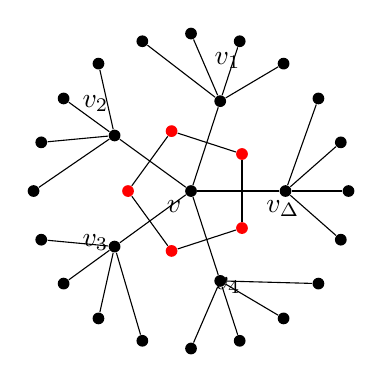
\begin{tikzpicture}
  \begin{scope}[shift={({0},{-2})}]
\foreach \i in {1,...,5}
\node[circle, fill=black, inner sep=1.5pt] (\i) at (72*\i:1.2) {};
\foreach \i in {1,...,5}
\node[circle, fill=red, inner sep=1.5pt] (\i\i) at (72*\i-36:0.8) {};

\foreach \i in {1,...,5}
    \foreach \j in {1,...,4}
    \node[circle, fill=black, inner sep=1.5pt] (5*\i+\j) at (72*\i+18*\j-36:2) {};
\node[circle, fill=black, inner sep=1.5pt] (0) at (0,0) {};
% edges
\foreach \i in {1,...,5}
        \draw (\i) -- (0);
\foreach \i[evaluate=\i as \m using int(\i+1)] in {1,...,4}
        \draw (\i\i) -- (\m\m);
\draw (55) -- (11);
\foreach \i in {1,...,5}
    \foreach \j in {1,...,4}
        \draw (\i) -- (5*\i+\j);
% labels
\foreach \i in {1,...,4}
\node[above] at (72*\i:1.5) {$v_{\i}$};
\node[anchor=north east] at (72*5:1.5) {$v_{\Delta}$};
    \node[anchor=north east] at (0,0) {$v$};
  \end{scope}
\end{tikzpicture}
  \end{subfigure} 
\end{figure}



\begin{claim}
  Let $Q =(C_{X},C_{Z})$ a good qLDPC CSS code. Then for any $g$ generator in $C_{Z}^{\perp}$ there is a logical gate compute $CX_{g}$ acting on at most $O(1)$ qubits. 
\end{claim}
\begin{proof}
  Recall that the generator matrix of $C_{Z}^\perp$ is the parity check matrix of $C_{Z}$. So we are looking for $\xi$ such that: 
  \begin{equation*}
    \begin{split}
      H_{Z}
      \begin{bmatrix}
        | \\
        | \\
        \xi \\
        | \\
        |
      \end{bmatrix} =
\begin{bmatrix}
        1 \\
        0 \\
        0 \\
        0 \\
        0
      \end{bmatrix}
    \end{split}
  \end{equation*}
  Assume that there is solution $\xi$ for the equations system. If $H_{z}$ is a parity check matrix of ltc code then $d(\xi,C_{Z}) = O(1)$ so we could picck some $z+\xi$ such that $z\in C_{Z}$ and having a solution that it's weight is $O(1)$.   %, then any $z + \xi$  where $z \in C_{Z}$ is also a solution.   
% \prod_{z_{r_i^{\prime}}}
  \begin{equation*}
    \begin{split}
      \sum_{r_{i},l_{j}}\ket{z_{r_i}}\ket{z_{l_j}} & = \sum_{z_{r_i^{\prime}}}\sum_{r_{i},l_{j}}\ket{z_{r_i}}\ket{z_{l_j}} \ket{ 0 + \xi[z_{r_{i^{\prime}}}]\cdot z_{r_{i}} } \sum_{z_{l_j^{\prime}}} \\ 
      x &
    \end{split}
  \end{equation*}

\end{proof}



\newcommand{\hashcode}{ checks-hashed }



\begin{definition}
  Let $\{h_{i} \}_{1}^{t}$ be the checks of $\Delta$-length code $C_{0}$. We say that $i$th bit and the $j$th bit collide if there a check $h$ such that $h_{i}=h_{j}=1$. We say that a $C_{0}$ is a \hashcode if:  
  \begin{equation*}
    \begin{split}
      \prbm{ i,j \text{ collide  }  }{ i, j \sim [\Delta]^{2} } < \frac{1}{2\Delta}
    \end{split}
  \end{equation*}
\end{definition}

\begin{claim}
  Suppose that $C_{0}^{\perp}$ is a \hashcode. Then $\left( C_{0}^{\otimes m} \right)^{\perp}$ is also a \hashcode. 
\end{claim}
\begin{proof}
  
  \begin{equation*}
    \begin{split}
      \prbm{X^{(m)}_{u,v}}{u,v\sim [n]^{2}} \le & \prbm{X^{(1)}_{u,v}}{u,v\sim [\Delta]^{2}} \cdot \prbm{X^{(m-1)}_{u,v} }{u,v\sim [n/\Delta]^{2}} \\ 
      \le & \frac{1}{2\Delta} \cdot \left( \frac{1}{2\Delta} \right)^{m-1} = \left( \frac{1}{2\Delta} \right)^{m}
    \end{split}
  \end{equation*}
\end{proof}

Consider the following decoder, we flip a bit if flipping it decrease the syndrome. Now observers that if a non faulty bit $i$ has been flip then it means that there is at least one faulty bit $j$ in the error $e$ that $i,j$ collide. Similarly if a faulty bit $i$ hasn't been flip then it means that there is another faulty bit $j$ that collide with him. In overall we conclude that the total number of incorrect flips made by the decoder is at most the number of collisions. 

\begin{equation*}
  \begin{split}
    \expp{\sum_{v \in e} \sum_{u \in [n]} X_{v,u}} \le |e|\cdot n \cdot \left( \frac{1}{2\Delta} \right)^{m} = \frac{|e|}{2^{m}}
  \end{split}
\end{equation*}

Now we are going to add a random error at weight $\frac{|e|}{2^{m}}$ to ensure that in the next iteration the $\frac{|e|}{2^{m-1}}$ error will distributed uniformly. Repeating for $\log_{2^{m-1}}$ rounds correct the error. (not exactly there is an error in each round that should be handled).   

\ctt{ We flip in over all $|e| \sum \frac{1}{2^{i}}  < 2|e| $ bits, so we would like to have $|e| \le d/4 $.} 


\ctt{ Yet we can do better, if $ e = z + \tilde{e}$ where $z$ commute with all our generators. }

\ctt{ And if it anticommute with only $l$ of them, then we have only $l$ errors. }


\begin{equation*}
  \begin{split}
    \Delta^{m}\le 1/p^{2}_{0} & \rightarrow \alpha \cdot 1/p^{2}_{0} , \frac{m}{2^{m}} \log \Delta 
  \end{split}
\end{equation*}


\begin{claim}
Let $H$ be a $|V|\times r$ binary parity check matrix of $\tilde{C}$. Also, let $G$ be a $\Delta$-regular graph. A bit assignment over $G$ edges $x$ will be said to be $\tilde{C}$-vertices-respect if the vector $z(x) \in \mathbb{F}_{2}^{|V|}$ which is defined as:
  \begin{equation*}
    z(x)_{v} = \begin{cases}
      1 & v \text{ sees at least one } 1\\
      0 & \text{otherwise}
    \end{cases}
  \end{equation*}
   is a codeword of $\tilde{C}$. Let $\Lambda$ be the set of all $\tilde{C}$-vertices-respect assignments. Then $|\Lambda| > (1-\varepsilon)2^{\rho |V|}$.
\end{claim}

\begin{proof} 
Any $x \in \Lambda$ is a solution for the following system of equations:
  \begin{equation*}
    \begin{split}
      z_{v} &= 1 + \prod_{ e \in v }{ \left( 1 - x_{e} \right) } \\
      Hz &= 0
    \end{split}
  \end{equation*}
\end{proof}

\begin{claim}
  Assume that $C_{0}$ is a $\Delta$-length code such that for any two non-trival codewords $c,c^{\prime}\in C_{0}$ we have that $c\cdot c^{\prime}=1$, and denote by $C = \mathcal{T}(G,C_{0})$. And let $\Lambda$ be a the set of all $\tilde{C}$-vertices-respect assignments where $\tilde{C}$ satisfies relation $R$. Then also $C \cap \Lambda$ satisfies $R$. 
\end{claim}





Let $\ket{f}$ be a codeword in $C_{X}$, and let $X_{g}$ be the indicator that equals $1$ if $f$ has support on $X_{g}$, and $0$ otherwise. Observes that applying $T^{\otimes}$ on $\ket{f}$ yilds the state: 
\begin{equation*}
  \begin{split}
    T^{\otimes n}\ket{f} & =  T^{\otimes n}\ket{\sum_{g} X_{g}g } = \exp \Big( i\pi/4 \sum_{g} X_{g}|g|  -  2 \cdot i \pi/4 \sum_{g,h} X_{g}X_{h}|g\cdot h| \\
    & +  4 \cdot i\pi/4 \sum_{g,h} X_{g}X_{h}X_{l}|g\cdot h \cdot l| -   8  \cdot i\pi/4 \cdot \text{ integers } \Big) \ket{f} \\
    & = \exp \Big( i\pi/4 \sum_{g} X_{g}|g|  -  2 \cdot \pi/4 \sum_{g,h} X_{g}X_{h}|g\cdot h| +  4 \cdot i\pi/4 \sum_{g,h} X_{g}X_{h}X_{l}|g\cdot h \cdot l| \Big) \ket{f}
  \end{split}
\end{equation*}

\section{Many to One.}
Assume that $f$ is supported on exactly one generator. Then we have that $T^{\otimes n}\ket{f}  = e^{i\pi|g|/4}\ket{f}$ Therefore, if $|g| = 4k+1$ then we are done.


\section{Using Quntum Error Correction Codes.}

Now assume that the code $C_{X}$ is the quantum Tanner code, denote by $G,A,B$ the group and the two generator sets that are used for constructing the square complex. 

\begin{claim} 
Consider $g,h$ that are supported on the same $v\in V$. We will call such a pair a source-sharing pair. Suppose that for any we have that $|g \cdot h|$ is even. Then there is a Clifford gate that computes $\ket{f} \mapsto \exp \Big(  -  i\pi \sum_{g,h \text{ source-sharing }} X_{g}X_{h}|g\cdot h|  \Big) \ket{f} $.
\end{claim}
%
%%\begin{claim}
%%  \label{claim:phase}
%%  The gate $\ket{f} \mapsto \exp \Big(   i\pi \sum_{g,h} X_{g}X_{h}X_{l}|g\cdot h \cdot l| \Big) \ket{f} $ is in the Clifford group.  
%%\end{claim}
%%
%%\begin{proof}
%%  Just decode $f$ and apply \textbf{CCZ} between any triple of qubits corresponding to the generators $g,h,l$ such that $g \cdot h \cdot l=_{2} 1$. Then encode the state again. Observes that \textbf{CCZ} is a Clifford gate, and by the fact that the code is a CSS code then the decoder and the encoder are both in the Clifford.
%%\end{proof}
%%
%
%
%\section{Fail Attempt.}
%
%
%In addition, let us assume the existence of $d \in G$ such that $d$ is non-identity and commutes with any element in $A \cup B$. Then, observe that multiplying by $d$ preserves adjacency on the complex. Namely, if $\{u,v\} \in E$ then also $\{du, dv\} \in E$. 
%
%Consider $\ket{f}$ such that if $X_g$ is not zero, and $g$ is associated with a local codeword $c \in C_A \otimes C_B$ on vertex $v$, then the generator associated with the local codeword $c$ on vertex $d \cdot v$ also supports $f$, denoted by $g'$. Thus, the exponent above becomes:
%
%\begin{equation*}
%  \begin{split}
%    & = \exp \Big( i\pi/4 \sum_{g} X_{g}|g|  -  2 \cdot \pi/4 \sum_{g,h \in G /a} X_{g}X_{h}|g\cdot h| + X_{g^{\prime}}X_{h^{\prime}}|g\cdot h |  \\
%    & +  4 \cdot i\pi/4 \sum_{g,h \in G/a} X_{g}X_{h}X_{l}|g\cdot h \cdot l| + X_{g^{\prime}}X_{h^{\prime}}X_{l^{\prime}}|g\cdot h \cdot l| \Big) \ket{f} \\
%    & = \exp \Big( i\pi/4 \sum_{g} X_{g}|g|  -  2 \cdot 2 \cdot \pi/4 \sum_{g,h \in G/a} X_{g}X_{h}|g\cdot h| +  2 \cdot 4 \cdot i\pi/4 \sum_{g,h \in G/a} X_{g}X_{h}X_{l}|g\cdot h \cdot l| \Big) \ket{f} \\
%    & = \exp \Big( i\pi/4 \sum_{g} X_{g}|g|  -  i\pi \sum_{g,h \in G/a} X_{g}X_{h}|g\cdot h|  \Big) \ket{f} 
%  \end{split}
%\end{equation*}
%
%\begin{figure}
%  \centering
%  \scalebox{0.1}{
%    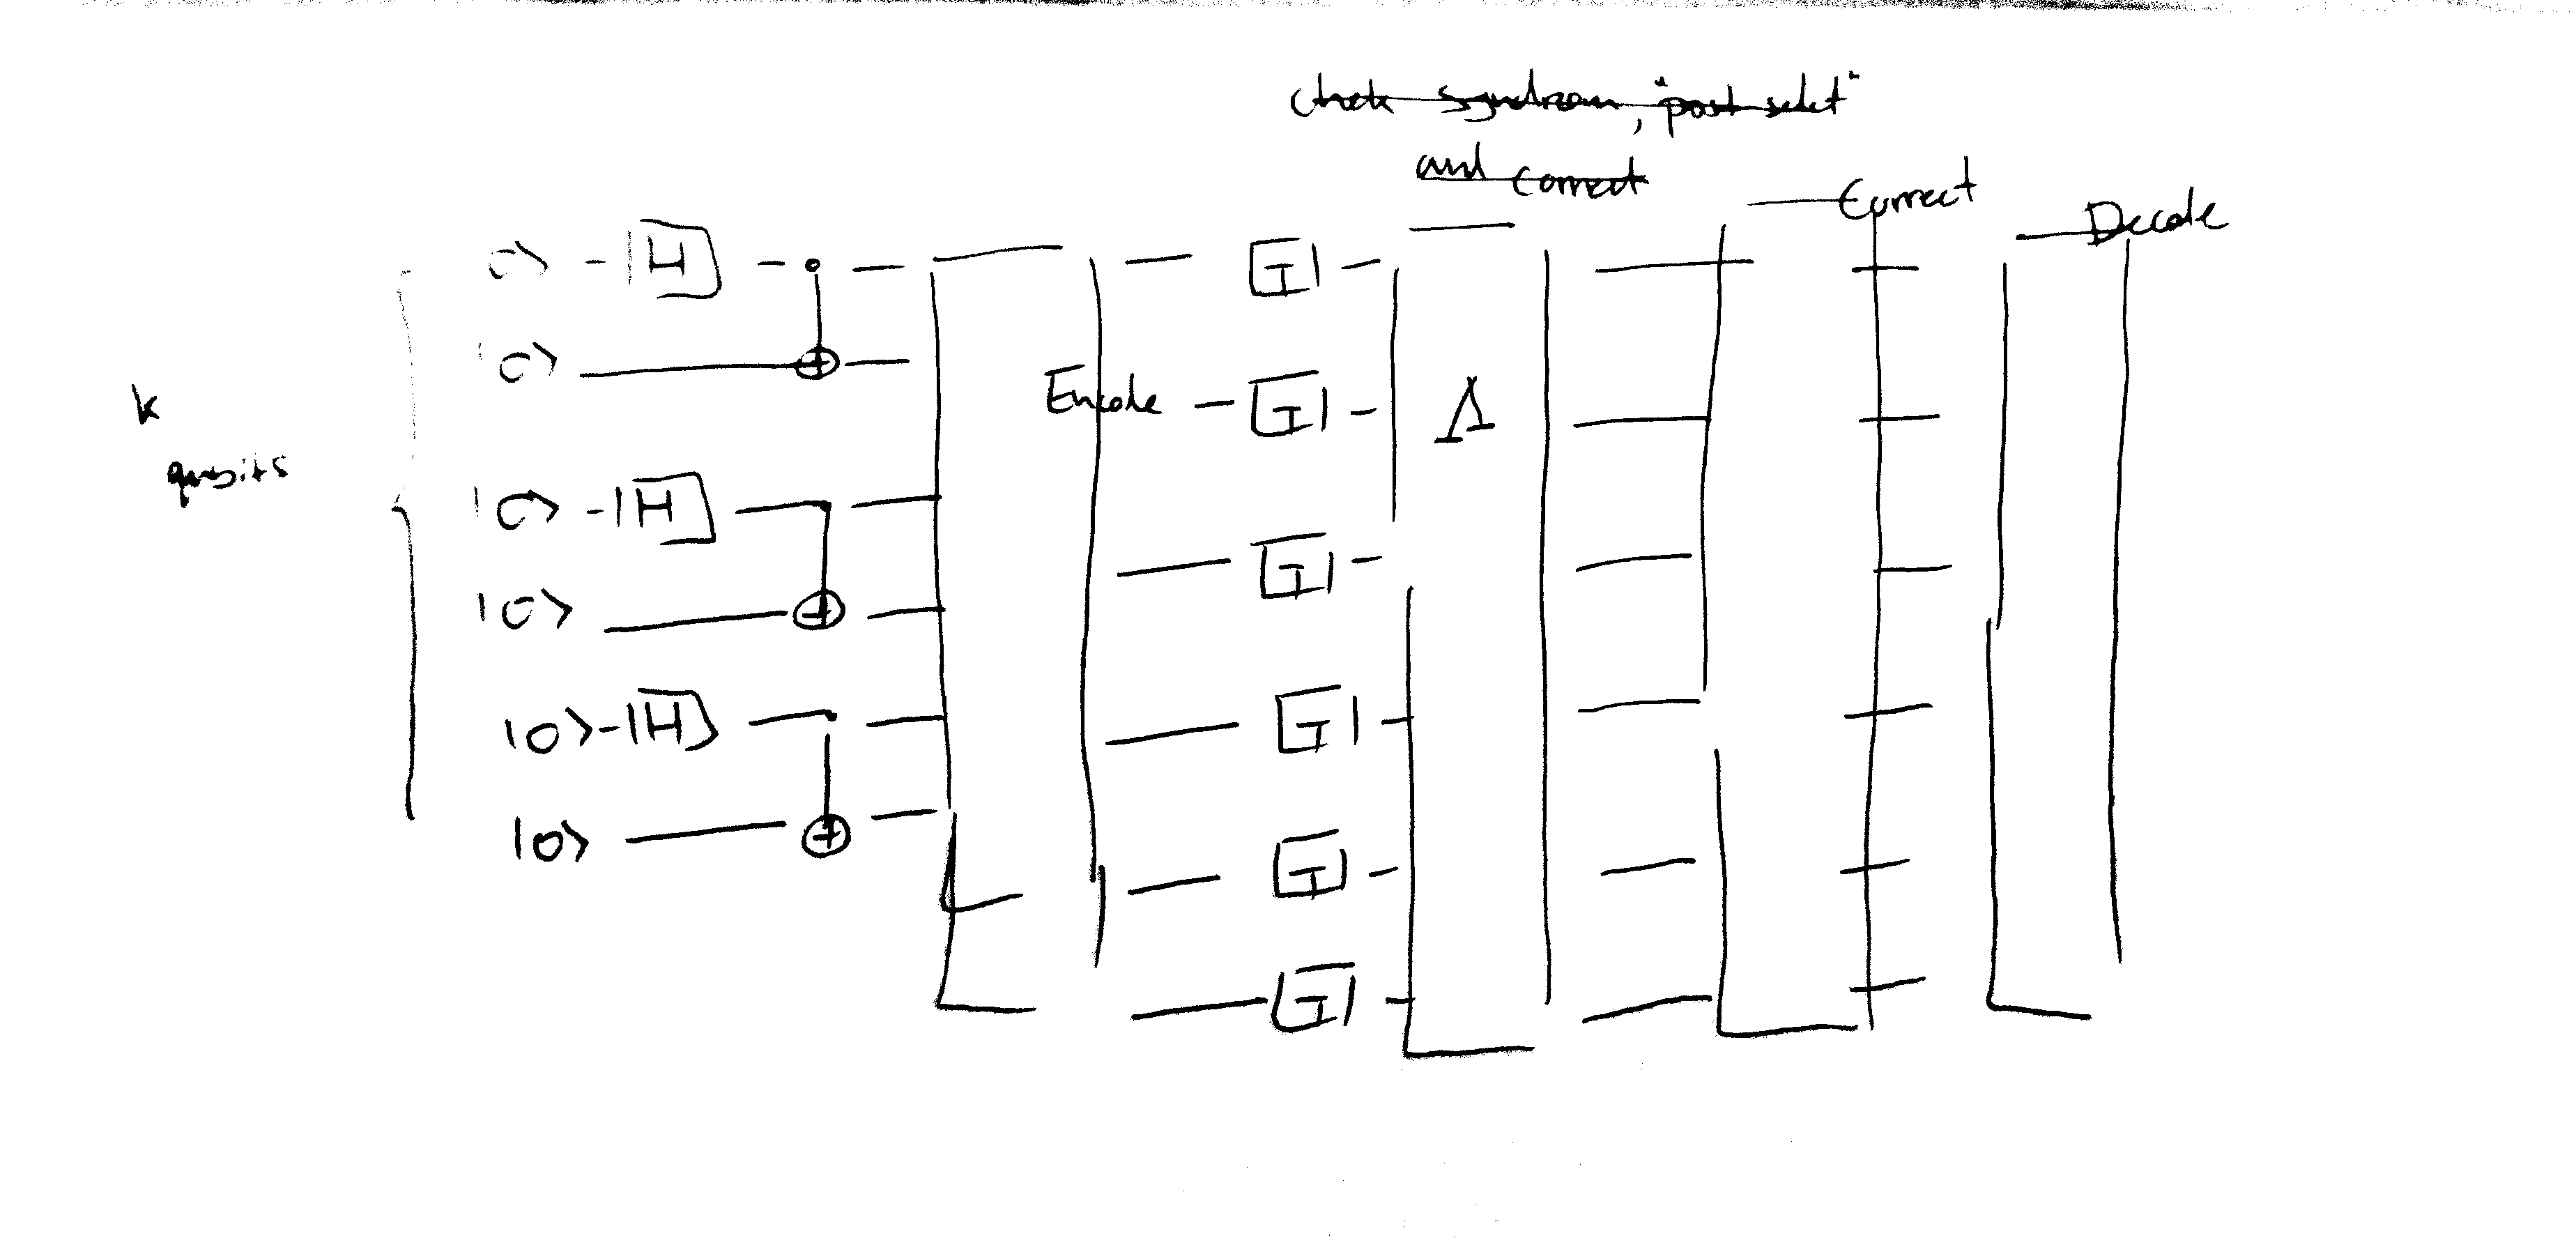
\includegraphics{distil.jpg-out.png}
%}
%  \caption{Quantum Circuit for distillation.}
%  \label{fig:circuit}
%\end{figure}
%
%\begin{claim}
%  \label{claim:phase}
%  The gate $\ket{f} \mapsto \exp \Big(  -  i\pi \sum_{g,h \in G/a} X_{g}X_{h}|g\cdot h|  \Big) \ket{f} $ is in the Clifford.  
%\end{claim}
%\begin{proof}
%Just decode $f$ and apply \textbf{CZ} between any pair of qubits corresponding to the generators $g,h$ such that $g \cap h = 1$. Then encode the state again. Observes that \textbf{CZ} is a Clifford gate, and by the fact that the code is a CSS code then the decoder and the encoder are both in the Clifford.
%\end{proof}
%Let's denote the circuit defined in \Cref{claim:phase} by $\Lambda$. So we have that:  
%\begin{equation*}
%  \begin{split}
%    \Lambda^{\dagger}\exp \Big( i\pi/4 \sum_{g} X_{g}|g|  & -  i\pi \sum_{g,h \in G/a} X_{g}X_{h}|g\cdot h|  \Big) \ket{f} \\
%= & \exp \Big( i\pi/4 \sum_{g} X_{g}|g|  \Big) \ket{f} 
%  \end{split}
%\end{equation*}
%
%Maybe what do we need is to arrange in some way $|g|+|g^{\prime}| = 4k+1$ and $\braket{g,f}= \braket{g^{\prime},f^{\prime}}$
%
%
%\begin{claim}
%  For any $m$ codewords $x_{1}..x_{m}$ there is a set of coordinates $I$ and $|I| < \alpha n$. Such that:  
%  \begin{equation*}
%    \begin{split}
%      \sum_{j \in [n]/I }x_{a}^{j}x_{b}^{j} = 0
%    \end{split}
%  \end{equation*}
%  For any pair $x_{a},x_{b}$. 
%\end{claim}
%
%\begin{claim}
%  For any $m$ codewords $x_{1}..x_{m}$ there is a set of coordinates $I$ and $|I| < \alpha n$. Such that:  
%  \begin{equation*}
%    \begin{split}
%      \sum_{a,b,j \in [n]/I }x_{a}^{j}x_{b}^{j} = 4k
%    \end{split}
%  \end{equation*}
%  For any pair $x_{a},x_{b}$. 
%\end{claim}
%









%\paragraph{What about concatination?} So, take a quantum good code. And consider a prasintion $k^{\prime}|k|m$ such that $k^{\prime} = \dim C_{Z}^{\perp}$ and $k = \dim C_{X}/C_{Z}^{\perp}$. Now concatinate with two genorthogonal codes, such that any logical bit of $k$ has wight of 1 module 8 and the others has weight 0.  



\begin{claim}
  Let $C_{A}$ and $C_{A^\prime}$ such that $C_{A^\prime} \subset C_{A}$. Then $\left(C_{A}^{\perp} \otimes C_{B}^{\perp}  \right)^{\perp}$, $ C_{A^{\prime}} \otimes C_{B^{\prime}}$ form a \textbf{CSS} code $C$ such there exists a subspace $V \subset C$ with effictive distance $d$. 
\end{claim}

\begin{proof}
  Idea. consider generators of the form $e_{0}\otimes g$. Any codeword  in their span is just a first row asssitmentd to a code word of $C_{A}$. If we assume less than linear number on that row then we will secucess to decode it, $+$ some other generators that we don't care about.   
\end{proof}



\begin{equation*}
  \begin{split}
    C_{X} & = \left( \left( C_{A} \otimes C_{0} \right)^{\perp} \otimes C_{0}^{\perp}  \right)^{\perp} \\ 
    C_{Z} & = \left( \left( C_{A} \otimes C_{0} \right) \otimes C_{0}  \right)^{\perp}
  \end{split}
\end{equation*}



\begin{claim}
  \label{claim:oneg}
  Let $C$ be a code at rate $\rho(C) > 7/8 $ has at least one codeword $x \in C$ , such that $|x| =_{8} 1 $.
\end{claim}

\begin{definition}
  We will say that a code $C$ is $(l,m)$-genorthogonal if there exists a generator set $G$ for $C$ such that for any $I \subset G$ such that $1 < |I| < l$ we have that:
  \begin{equation*}
    \begin{split}
      \sum_{i \in [n]}\prod_{g_{j}\in I \subset G}g_{j}^{i} =_{m} 0 
    \end{split}
  \end{equation*}
\end{definition}

\begin{claim} \label{claim:goodgen} 
  If there exists a single $(l,m)$-genorthogonal code for a finite length $\Delta$, then there is a family of $(l,m)$-genorthogonal good codes. Moreover, if there exists a generator in $C_0$ of weight $|\cdot|_m = 1$, then there exists a family that also has at least one generator of weight $|\cdot|_m = 1$.
\end{claim}
\begin{proof}
  Denote by $C_{0} = \Delta[1,\rho_{0}, \delta_{0}]$ an $(l,m)$-genorthogonal code and observes that for any $C = [n,\rho n, \delta n]$ the tensor code $C_{0}\otimes C = [\Delta n, \rho_{0} \rho \Delta n, \delta_{0} \delta \Delta n]$ is also $(l,m)$-genorthogonal code. 

  For the seconed part of the claim, Choose $C$ to be a good code with rate $> \left(2^{m}-1\right)/2^{m}$ by \Cref{claim:oneg} there is at least on codeword $c$ in $C$ such that $|c| =_{m} 1$.

  So pick the base for $C_{0}\otimes C$ such the first generator is $g_{0} \otimes c$ where $g_{0}$ denote a generator of $C_{0}$ satisfies $|g_{0}| =_{m} 1$. 
    Then $|g_{0} \otimes c | = |g_{0}| \cdot |c| =_{m} 1$.  
\end{proof}

\begin{claim}
  Suppose that there exists $(m+1,m)$-genorthogonal code, such that any generator of it has weight $| \cdot | =_{m} 1$ then there exists also a family of good $(m+1,m)$-genorthogonal codes such that a liner portion of his generators $g$ have weight $|g| =_{m} 1$. 
\end{claim}

\begin{proof}  
  Denote by $C_{0}$ a finte $(m+1,m)$-genorthogonal code, such that any generator of it has weight $| \cdot | =_{m} 1$. Let $C$ be a good $(m+1,m)$-genorthogonal code with generator $c$ such that $|c| =_{m} 1$, the existence of which is given by \Cref{claim:goodgen}. Denote its rate by $\rho$. If $C$ has more than $\rho/m \cdot n$ generators at weight $| \cdot | =_{m} 1$ then we are done. Otherwise, by the pigeonhole principle, there is an $i$ such that more than $\rho/m$ portion of the generators are at weight $ |\cdot| =_{m} i$. Denote them by $g_{1},g_{2},g_{3}, \dots, g_{m}$.

  Define the set $g_{1}^{^\prime},g_{2}^{\prime}..g_{m}^{\prime}$ as   
  \begin{equation*}
    \begin{split}
      g^{\prime}_{t} & = c + \sum_{j=t}^{t+m}g_{j} \\
      & \Rightarrow |g^{\prime}_{t+1}| = |c| + \sum_{t}{ |g_{j}| } + \sum_{|I|<l+1}\left|\prod_{g \in I  } \alpha_{\star} g \right| \\
      & =_{m} c + m\cdot i =_{m} c =_{m} 1  
    \end{split}
  \end{equation*}  
Now take $C_0 \otimes C$, and set the new generator set to be $g^0_i \otimes g'_j$. And it's easy to verify that we got the code we wanted.
\end{proof}

\begin{claim} \label{claim:code}
  There exists, a good LDPC code (classic) $C$ such that $C^{\perp}$ is also a good code and a generator set $G$, for exists $G^{\prime} \subset G$ and $|G^{\prime}| = \Theta( |G|)$ such:  
  \begin{enumerate}
    \item For any pair $x \neq y \in G^{\prime} \rightarrow x\cdot y =_{8} 0$
    \item For any triple $x\neq y,z \in G^{\prime} \rightarrow \sum_{i}x_{i}y_{i}z_{i} =_{8} 0$
    \item For any $x \in G^{\prime} \rightarrow |x| =_{8} 1$  
  \end{enumerate}
\end{claim}


\begin{claim}  
  There is $n \rightarrow \Theta(n)$ magic states distillation into a binary qldpc code with $\Theta(\sqrt{n})$ distance, and therefore with asymptotic overhead approaching $1$ 
\end{claim}

\begin{proof}
For the encoding we are going to use the hyperproduct code defined in \cite{Tillich_2014}. Let $C$ be the code given by \Cref{claim:code} and consider the hyperproduct of $C$ with itself $Q = Q(C \times_{H} C)$. In addition, denote by $C_{X},C_{Z}$ the CSS representation of $Q$. 

By the fact that $C^\perp$ is also a good code, then $Q$ is a positive rate, square root distance code. Let $\rho$ be the rate of $C$ and $1 - \rho$ be the rate of $C^{\perp}$. As $\rho > 0$, then one can find $I \subset [n]$ coordinates such that for any $i \in I$ the indicator $e_{i} \not\in C^{\perp}$. Hence, it holds from \cite{Tillich_2014} that any vector of the form $e_{i}\otimes x$ is a codeword of $C_{X}/C_{Z}^{\perp}$.

Denote by $\rho^{\prime}$ the portion of $G^{\prime}$ as defined in \Cref{claim:code}, and define $S$ to be: 
\begin{equation*}
  \begin{split}
    S = \left\{ e_{i} \otimes x| e_{i} \not\in C^{\perp}, x \in G^{\prime} \right\}
  \end{split}
\end{equation*}
Observes that $|S| = \rho^{\prime}\rho n^{2}$ and in addition $S$ satisfies the properties in \Cref{claim:code}. Denote by $f$ a codeword supported only on $S$ and denote by $X_{s}$ the indecator that indicate that $s$ supports $f$. Thus:  
\begin{equation*}
  \begin{split}
    T^{\otimes n}\ket{f}  = \exp \Big( i\pi/4 & \sum_{g} X_{g} \overbrace{|g|}^{8k+1}  \\ 
    & -  2 \cdot i \pi/4  \overbrace{\sum_{g,h} X_{g}X_{h}|g\cdot h|}^{8k} \\ 
  & +  4 \cdot i\pi/4 \overbrace{ \sum_{g,h} X_{g}X_{h}X_{l}|g\cdot h \cdot l| }^{8k } \Big) \ket{f} \\
  & \\ 
  =   \exp \Big( i\pi/4 & \sum_{g \in S} X_{g} \Big) \ket{f}
      \end{split}
\end{equation*}
Therefore we can, generate the enocded (\ctt{For now without spanning on on $C_{Z }^{\perp}$} ) product of $T^{\otimes|S|}\ket{+}^{|S|}$:
\begin{equation*}
  \begin{split}
    \prod_{s \in S} \Big( \ket{0} + \exp \left( i\pi/4 \right) \ket{s} \Big)
  \end{split}
\end{equation*}

\ctt{What is left: 
  \begin{enumerate}
    \item Show that one can generate $ \prod_{s \in S} \Big( \ket{C_{Z}^{\perp}} + \exp \left( i\pi/4 \right) \ket{C_{Z}^{\perp} + s} \Big)$ without propagate the errors. I think I know how to do it.
    \item Compute a threshold $p_{0}$ for using Baravi construction.
  \end{enumerate}
}

Thus we have that $\gamma = \log(n/k)/\log(d) =  \log(n/|S|)/\log(\Theta(\sqrt{n})) \rightarrow 0$ and the overhead growes as $\log^{\gamma}(n) \rightarrow 1$ \cite{bravyi2012magic}, \cite{meier2012magicstate}.
\end{proof}

% Triorthogonal

\fi

\printbibliography

\end{document}







